\documentclass[11pt,a4paper]{article}
\usepackage[utf8]{inputenc}
\usepackage[margin=2.5cm]{geometry}
\usepackage{graphicx}
\usepackage{tikz}
\usepackage{enumitem}
\usepackage{xcolor}
\usepackage{hyperref}
\usepackage{fancyhdr}
\usepackage{booktabs}
\usepackage{float}

\usetikzlibrary{shapes.geometric, arrows.meta, positioning, calc, backgrounds, fit}

\pagestyle{fancy}
\fancyhf{}
\rhead{Demo Priorities}
\lhead{Federated ICS Threat Correlation Engine}
\rfoot{Page \thepage}

\hypersetup{
    colorlinks=true,
    linkcolor=blue,
    urlcolor=blue,
    citecolor=blue
}

\definecolor{critical}{RGB}{220,53,69}
\definecolor{high}{RGB}{255,193,7}
\definecolor{medium}{RGB}{40,167,69}
\definecolor{low}{RGB}{108,117,125}

\title{\textbf{Federated ICS Threat Correlation Engine}\\
\large Demo Priorities for November 30, 2025}
\author{Industrial Control Systems Security Team}
\date{October 14, 2025}

\begin{document}

\maketitle
\thispagestyle{fancy}

\begin{abstract}
This document defines the absolute essential features that must be demonstrated by November 30, 2025 to prove the unique value proposition of the Federated ICS Threat Correlation Engine. The focus is on delivering a working prototype that demonstrates federated learning, multi-layered detection, attack prediction, and privacy preservation.
\end{abstract}

\tableofcontents
\newpage


\section{Overview}

This document defines the absolute essential features that must be demonstrated by November 30, 2025 to prove the unique value proposition of the Federated ICS Threat Correlation Engine. The system aims to enable privacy-preserving collaborative defense across multiple industrial facilities through federated learning, while providing real-time threat detection and proactive attack prediction.

\subsection{Key Objectives}

\begin{itemize}[leftmargin=*]
    \item Demonstrate federated learning enabling collaborative defense across 3 simulated facilities
    \item Prove multi-layered detection with LSTM, Isolation Forest, and Physics Rules working in parallel
    \item Show attack prediction using Graph Neural Networks with MITRE ATT\&CK for ICS
    \item Validate privacy preservation through differential privacy and data sovereignty
    \item Provide visual proof through real-time dashboard
\end{itemize}

\section{MUST HAVE - Core Demo Requirements}

\subsection{Federated Learning (THE KILLER FEATURE)}

\textbf{Priority:} \textcolor{critical}{CRITICAL} \\
\textbf{Why it's critical:} This is the ONLY unique differentiator vs competitors

\subsubsection{Must Demonstrate}

\begin{itemize}[leftmargin=*]
    \item 3 simulated facilities (Facility A, B, C)
    \item FL Server coordinating rounds
    \item Visual proof that:
    \begin{itemize}
        \item Facility A gets attacked
        \item FL round triggered
        \item Model updated and distributed
        \item Facilities B \& C now detect the same attack
    \end{itemize}
    \item Show timing: ``6-24 hours'' vs ``weeks/months'' for traditional sharing
\end{itemize}


\subsubsection{Demo Scenario}

\begin{enumerate}[leftmargin=*]
    \item Show Facility A detecting novel attack
    \item Trigger FL round (show it happening)
    \item Show Facilities B \& C receiving updated model
    \item Replay same attack on Facility B $\rightarrow$ Now detected!
    \item Show dashboard: ``All facilities protected in 6 hours''
\end{enumerate}

\textbf{Why essential:} Without this, the system is just another ICS security tool.

\subsection{Real-Time Detection (PROOF IT WORKS)}

\textbf{Priority:} \textcolor{critical}{CRITICAL} \\
\textbf{Why it's critical:} Need to show the system actually detects threats with multiple methods

\subsubsection{Must Demonstrate}

THREE working detection methods running in parallel:

\begin{itemize}[leftmargin=*]
    \item \textbf{LSTM Autoencoder} - Behavioral anomalies (temporal patterns)
    \item \textbf{Isolation Forest} - Point anomalies (sudden outliers)
    \item \textbf{Physics Rules Engine} - Process violations (safety constraints)
\end{itemize}

Additional requirements:
\begin{itemize}[leftmargin=*]
    \item Real-time alerts appearing on dashboard ($<$30 seconds)
    \item Clear visualization of anomaly detection
    \item Correlation showing multiple sources agree
\end{itemize}

\subsubsection{Why All Three Methods}

\begin{itemize}[leftmargin=*]
    \item \textbf{LSTM:} Detects subtle behavioral changes over time
    \item \textbf{Isolation Forest:} Catches sudden spikes and outliers LSTM might miss
    \item \textbf{Physics Rules:} Validates against known safety constraints
    \item \textbf{Together:} Reduces false positives, increases confidence
\end{itemize}


\subsubsection{Detection Architecture}

\begin{figure}[H]
\centering
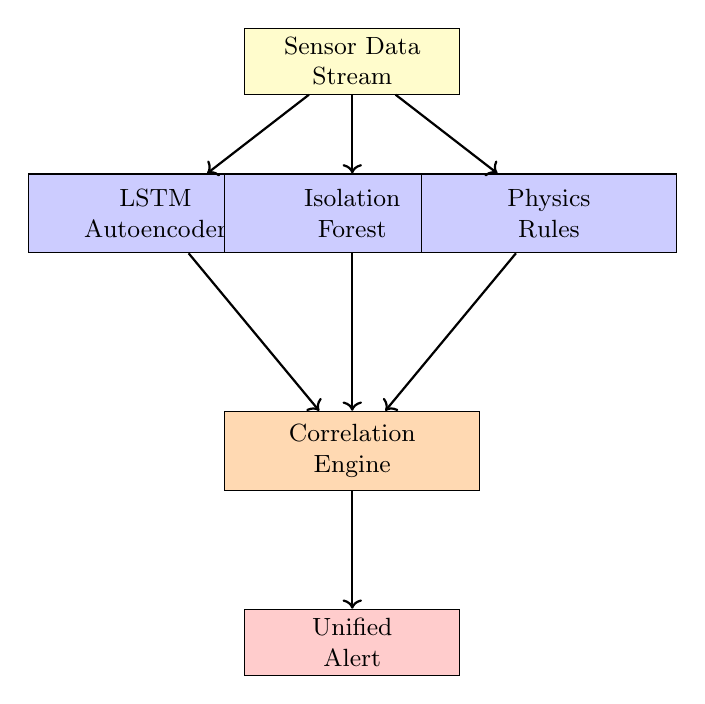
\begin{tikzpicture}[
    node distance=1.5cm,
    detector/.style={rectangle, draw, fill=blue!20, text width=3cm, align=center, minimum height=1cm, font=\small},
    data/.style={rectangle, draw, fill=yellow!20, text width=2.5cm, align=center, minimum height=0.8cm, font=\small},
    engine/.style={rectangle, draw, fill=orange!30, text width=3cm, align=center, minimum height=1cm, font=\small},
    alert/.style={rectangle, draw, fill=red!20, text width=2.5cm, align=center, minimum height=0.8cm, font=\small}
]

\node[data] (sensor) {Sensor Data\\Stream};

\node[detector, below left=1cm and -0.5cm of sensor] (lstm) {LSTM\\Autoencoder};
\node[detector, below=1cm of sensor] (if) {Isolation\\Forest};
\node[detector, below right=1cm and -0.5cm of sensor] (physics) {Physics\\Rules};

\node[engine, below=2cm of if] (corr) {Correlation\\Engine};

\node[alert, below=1.5cm of corr] (output) {Unified\\Alert};

\draw[->, thick] (sensor) -- (lstm);
\draw[->, thick] (sensor) -- (if);
\draw[->, thick] (sensor) -- (physics);

\draw[->, thick] (lstm) -- (corr);
\draw[->, thick] (if) -- (corr);
\draw[->, thick] (physics) -- (corr);

\draw[->, thick] (corr) -- (output);

\end{tikzpicture}
\caption{Multi-Layered Detection Architecture}
\end{figure}

\subsubsection{Demo Scenario}

\begin{enumerate}[leftmargin=*]
    \item Show normal operation (green, all good)
    \item Inject Modbus attack with sudden value spike
    \item Isolation Forest detects outlier immediately ($<$5 seconds)
    \item LSTM detects behavioral anomaly (within 30 seconds)
    \item Physics rules violated (temperature out of range)
    \item Correlation engine: ``Detected by all 3 sources - CRITICAL''
    \item Alert appears on dashboard with high confidence (0.95)
\end{enumerate}

\textbf{Why essential:}
\begin{itemize}[leftmargin=*]
    \item Proves robust multi-layered detection
    \item Shows defense-in-depth approach
    \item Demonstrates low false positive rate (all 3 agree = real threat)
\end{itemize}


\subsection{Dashboard Visualization (SHOW, DON'T TELL)}

\textbf{Priority:} \textcolor{critical}{CRITICAL} \\
\textbf{Why it's critical:} Visual proof is more convincing than logs

\subsubsection{Must Have Pages}

\begin{itemize}[leftmargin=*]
    \item \textbf{Alerts Dashboard} - Real-time alert feed
    \item \textbf{FL Status Page} - Show rounds, clients, model updates
    \item \textbf{System Overview} - 3 facilities, their status
\end{itemize}

\subsubsection{Minimum Viable Requirements}

\begin{itemize}[leftmargin=*]
    \item Simple, clean interface (doesn't need to be fancy)
    \item Real-time updates (WebSocket)
    \item Clear status indicators (green/red)
\end{itemize}

\subsubsection{Demo Scenario}

\begin{enumerate}[leftmargin=*]
    \item Show dashboard with 3 facilities
    \item Facility A: Alert appears (red)
    \item FL Status: Round in progress
    \item Facilities B \& C: Models updating
    \item All facilities: Now protected (green)
\end{enumerate}

\textbf{Why essential:} Makes the abstract concept concrete and visible.

\subsection{Privacy Preservation (TRUST FACTOR)}

\textbf{Priority:} \textcolor{high}{HIGH} \\
\textbf{Why it's critical:} Addresses the ``why not just share data?'' question

\subsubsection{Must Demonstrate}

\begin{itemize}[leftmargin=*]
    \item Show that raw data stays local
    \item Only model weights transmitted ($\sim$10 MB)
    \item Differential privacy applied ($\varepsilon=2.0$, $\delta=10^{-5}$)
\end{itemize}

\subsubsection{Demo Scenario}

\begin{enumerate}[leftmargin=*]
    \item Show Facility A's sensitive data (temperature, pressure)
    \item Show FL round: ``Transmitting weights only (10 MB)''
    \item Show privacy metrics: ``$\varepsilon=2.0$ guarantee''
    \item Emphasize: ``Raw data never left Facility A''
\end{enumerate}

\textbf{Why essential:} This is what makes FL acceptable for critical infrastructure.


\subsection{Attack Prediction (WOW FACTOR)}

\textbf{Priority:} \textcolor{critical}{CRITICAL} \\
\textbf{Why it's critical:} Proactive defense - predicts attacker's next move

\subsubsection{Must Demonstrate}

\begin{itemize}[leftmargin=*]
    \item Graph Neural Network (GAT) predicting next attack steps
    \item MITRE ATT\&CK for ICS technique mapping
    \item Probability scores for next likely techniques
    \item Visual graph showing attack progression
\end{itemize}

\subsubsection{Demo Scenario}

\begin{enumerate}[leftmargin=*]
    \item Show current attack: T0846 (Remote System Discovery)
    \item GNN predicts next steps:
    \begin{itemize}
        \item T0843 (Program Download) - 67\% probability
        \item T0800 (Lateral Movement) - 23\% probability
        \item T0858 (Change Operating Mode) - 10\% probability
    \end{itemize}
    \item Show target asset: PLC-REACTOR-01
    \item Show timeframe: ``15-60 minutes''
    \item Attacker proceeds with T0843 $\rightarrow$ System predicted it!
    \item Show proactive defense: ``Blocked based on prediction''
\end{enumerate}

\textbf{Why essential:} Shifts from reactive to proactive defense - unique competitive advantage.

\subsubsection{Federated Learning Enhancement}

\begin{itemize}[leftmargin=*]
    \item GNN learns attack patterns from all facilities
    \item When Facility A sees new attack chain, all facilities learn it
    \item Improves prediction accuracy across the network
\end{itemize}

\section{NICE TO HAVE - Enhances Demo}

\subsection{Protocol Anomaly Detection}

\textbf{Priority:} \textcolor{medium}{MEDIUM} \\
\textbf{Why it's nice:} Additional layer but not essential with 3 methods already

\textbf{If you have time:}
\begin{itemize}[leftmargin=*]
    \item Deep packet inspection for protocol violations
    \item Malformed message detection
    \item Unusual command sequences
\end{itemize}

\textbf{Skip for MVP:} Focus on LSTM, Isolation Forest, and Physics Rules first


\subsection{Multiple Protocols}

\textbf{Priority:} \textcolor{medium}{MEDIUM} \\
\textbf{Why it's nice:} Shows versatility but not essential

\begin{itemize}[leftmargin=*]
    \item \textbf{Minimum:} Modbus only
    \item \textbf{Nice to have:} + DNP3
    \item \textbf{Skip for MVP:} OPC-UA, S7
\end{itemize}

\section{CAN SKIP - Not Essential for Demo}

\subsection{Advanced Forensics}
Time-travel investigation nice but not essential. Can be basic query interface for MVP.

\subsection{Red Team Simulator}
Automated testing not essential. Manual attack injection sufficient.

\subsection{MongoDB}
Can use PostgreSQL for logs. Reduces complexity (but keep if time allows).

\subsection{Multiple Protocols Beyond Modbus}
DNP3, OPC-UA, S7 can wait. Modbus sufficient for demo.

\section{Absolute Minimum Demo}

\subsection{The 3-Minute Demo Script}

\begin{enumerate}[leftmargin=*]
    \item \textbf{SHOW:} 3 facilities running, all green
    \begin{itemize}
        \item ``Three power plants, each with their own ICS''
    \end{itemize}
    
    \item \textbf{ATTACK:} Facility A gets hit
    \begin{itemize}
        \item ``Novel Modbus attack on Facility A''
        \item Alert appears, LSTM detects anomaly
    \end{itemize}
    
    \item \textbf{FEDERATED LEARNING:} Round triggered
    \begin{itemize}
        \item ``FL round initiated - facilities learning together''
        \item Show FL status: training, aggregating, distributing
    \end{itemize}
    
    \item \textbf{PROTECTION:} Facilities B \& C now protected
    \begin{itemize}
        \item ``6 hours later, all facilities protected''
        \item Replay attack on Facility B $\rightarrow$ Immediately detected!
    \end{itemize}
    
    \item \textbf{PRIVACY:} Emphasize data sovereignty
    \begin{itemize}
        \item ``Facility A's data never left their premises''
        \item Show: Only 10 MB weights transmitted
    \end{itemize}
    
    \item \textbf{COMPARISON:} Traditional vs Federated
    \begin{itemize}
        \item ``Traditional: Weeks to share threat intelligence''
        \item ``Federated: 6 hours, automatic, privacy-preserving''
    \end{itemize}
\end{enumerate}


\subsection{What This Proves}

\begin{itemize}[leftmargin=*]
    \item Detection works
    \item FL works
    \item Privacy preserved
    \item Faster than competitors
    \item Collaborative defense
\end{itemize}

\section{Implementation Priority Order}

\subsection{Week 1-2: Foundation + Detection}

\begin{enumerate}[leftmargin=*]
    \item Docker Compose setup
    \item Kafka + PostgreSQL + IoTDB
    \item Modbus simulator
    \item LSTM Autoencoder working
    \item Isolation Forest working
    \item Physics Rules working
    \item Correlation Engine
    \item Basic alerts
\end{enumerate}

\subsection{Week 3: Federated Learning (CRITICAL)}

\begin{enumerate}[leftmargin=*]
    \item FL Server (Flower)
    \item 3 FL Clients
    \item Differential Privacy (Opacus)
    \item Model distribution working
    \item FL round completes successfully
\end{enumerate}

\subsection{Week 4: Attack Prediction \& Graph}

\begin{enumerate}[leftmargin=*]
    \item Neo4j MITRE ATT\&CK graph
    \item Graph Neural Network (GAT) implementation
    \item Attack prediction service
    \item Technique mapping and API endpoints
\end{enumerate}

\subsection{Week 5: Dashboard}

\begin{enumerate}[leftmargin=*]
    \item Alerts page
    \item FL status page
    \item Attack graph visualization (D3.js)
    \item System overview
    \item Real-time updates
\end{enumerate}

\subsection{Week 6: Integration \& Demo}

\begin{enumerate}[leftmargin=*]
    \item Connect all components end-to-end
    \item 3 demo scenarios (detection, FL, prediction)
    \item Video walkthrough
    \item Documentation
    \item Polish and practice
\end{enumerate}


\section{Success Criteria for Demo}

\subsection{Minimum Success}

\begin{itemize}[leftmargin=*]
    \item FL round completes with 3 facilities
    \item Detection works (at least 2 of 3 methods)
    \item Dashboard shows it visually
    \item Can demonstrate collaborative defense
\end{itemize}

\subsection{Good Success}

\begin{itemize}[leftmargin=*]
    \item Above + all 3 detection methods working (LSTM, IF, Physics)
    \item Above + correlation engine combining signals
    \item Above + attack prediction (GNN)
    \item Above + polished dashboard
    \item Above + clear privacy demonstration
\end{itemize}

\subsection{Excellent Success}

\begin{itemize}[leftmargin=*]
    \item Above + Isolation Forest
    \item Above + multiple protocols
    \item Above + forensics
    \item Above + advanced correlation
\end{itemize}

\section{The One Thing That MUST Work}

\textbf{If you can only get ONE thing working perfectly:}

\subsection{Federated Learning Demonstration}

Show the following:
\begin{enumerate}[leftmargin=*]
    \item Facility A detects attack
    \item FL round triggered
    \item All facilities learn
    \item Facility B now protected
    \item Data stayed local
\end{enumerate}

\textbf{This alone proves your unique value proposition.}


\section{Feature Comparison Matrix}

\begin{table}[H]
\centering
\small
\begin{tabular}{@{}lcccc@{}}
\toprule
\textbf{Feature} & \textbf{Priority} & \textbf{Complexity} & \textbf{Impact} & \textbf{Include?} \\ \midrule
Federated Learning & CRITICAL & High & Very High & \textcolor{critical}{MUST} \\
LSTM Detection & CRITICAL & Medium & High & \textcolor{critical}{MUST} \\
Isolation Forest & CRITICAL & Low & High & \textcolor{critical}{MUST} \\
Physics Rules & CRITICAL & Low & High & \textcolor{critical}{MUST} \\
Correlation Engine & CRITICAL & Low & Very High & \textcolor{critical}{MUST} \\
Dashboard (Basic) & HIGH & Medium & High & \textcolor{critical}{MUST} \\
Privacy Demo & HIGH & Low & High & \textcolor{critical}{MUST} \\
Attack Prediction (GNN) & CRITICAL & High & Very High & \textcolor{critical}{MUST} \\
Neo4j & HIGH & Medium & High & \textcolor{critical}{MUST} \\
MongoDB & LOW & Low & Low & \textcolor{low}{SKIP} \\
Multiple Protocols & LOW & Medium & Low & \textcolor{low}{SKIP} \\
Forensics & LOW & Medium & Low & \textcolor{low}{SKIP} \\ \bottomrule
\end{tabular}
\caption{Feature Priority Matrix}
\end{table}

\section{Risk Mitigation}

\subsection{If Federated Learning is Delayed}

\textbf{Fallback:} Show simulated FL with manual model updates \\
\textbf{Impact:} Still demonstrates concept, less impressive

\subsection{If One Detection Method Fails}

\textbf{Fallback:} Demonstrate with 2 out of 3 methods (any combination works) \\
\textbf{Impact:} Still shows multi-layered approach, slightly less impressive \\
\textbf{Note:} Having all 3 working is ideal but not critical - 2 methods sufficient

\subsection{If Dashboard is Behind}

\textbf{Fallback:} Use command-line demo with logs \\
\textbf{Impact:} Less visual but proves functionality

\subsection{If Integration Fails}

\textbf{Fallback:} Demonstrate components separately \\
\textbf{Impact:} Less impressive but shows individual capabilities


\section{Demo Scenarios}

\subsection{Scenario 1: Multi-Layered Detection + FL}

\subsubsection{Setup}
\begin{itemize}[leftmargin=*]
    \item 3 facilities running normally
    \item All showing green status
    \item All 3 detection methods active
\end{itemize}

\subsubsection{Execution}

\begin{enumerate}[leftmargin=*]
    \item \textbf{Inject Modbus write attack on Facility A} (sudden value spike)
    \item \textbf{Isolation Forest detects outlier} ($<$ 5 seconds)
    \begin{itemize}
        \item ``Anomaly score: 0.85 - Sudden spike detected''
    \end{itemize}
    \item \textbf{LSTM detects behavioral anomaly} ($<$ 30 seconds)
    \begin{itemize}
        \item ``Reconstruction error: 0.92 - Pattern deviation detected''
    \end{itemize}
    \item \textbf{Physics rules violated} (temperature out of safe range)
    \begin{itemize}
        \item ``CRITICAL: Temperature 380°C exceeds max 350°C''
    \end{itemize}
    \item \textbf{Correlation Engine combines all three}
    \begin{itemize}
        \item ``HIGH CONFIDENCE ALERT: Detected by 3/3 sources''
        \item Confidence: 0.95, Severity: CRITICAL
    \end{itemize}
    \item \textbf{Alert displayed on dashboard} with all source details
    \item \textbf{FL round triggered automatically}
    \item Show FL progress: training, aggregating, distributing
    \item \textbf{Replay same attack on Facility B}
    \item All 3 detection methods now catch it immediately
    \item Show privacy metrics: only weights transmitted
\end{enumerate}

\subsubsection{Duration}
4-6 minutes

\subsubsection{Key Message}
\begin{itemize}[leftmargin=*]
    \item ``Defense in depth: Multiple detection layers working together''
    \item ``One facility's experience protects all others within hours''
    \item ``Low false positives: All 3 methods agree = real threat''
\end{itemize}


\subsection{Scenario 2: Attack Prediction in Action}

\subsubsection{Setup}
\begin{itemize}[leftmargin=*]
    \item System running normally
    \item MITRE ATT\&CK graph loaded in Neo4j
    \item GNN model trained on attack sequences
\end{itemize}

\subsubsection{Execution}

\begin{enumerate}[leftmargin=*]
    \item Attacker performs reconnaissance (T0846: Remote System Discovery)
    \item System detects and alerts
    \item GNN analyzes current state and predicts next steps:
    \begin{itemize}
        \item T0843 (Program Download) - 67\% probability
        \item T0800 (Lateral Movement) - 23\% probability
        \item T0858 (Change Operating Mode) - 10\% probability
    \end{itemize}
    \item Show attack graph visualization with predicted path highlighted
    \item Show target asset: PLC-REACTOR-01
    \item Show timeframe: ``Next step expected in 15-60 minutes''
    \item Proactive defense: Increase monitoring on PLC-REACTOR-01
    \item Attacker attempts T0843 (Program Download)
    \item System: ``Predicted attack confirmed! Blocking...''
    \item Show how prediction enabled proactive defense
\end{enumerate}

\subsubsection{Duration}
3-5 minutes

\subsubsection{Key Message}
``Don't just react to attacks - predict and prevent them''

\subsubsection{Federated Learning Enhancement}
\begin{itemize}[leftmargin=*]
    \item Show that GNN learned this attack pattern from Facility A
    \item Now all facilities can predict this attack chain
    \item Demonstrate collaborative intelligence improving predictions
\end{itemize}


\subsection{Scenario 3: Multi-Facility Collaborative Defense}

\subsubsection{Setup}
\begin{itemize}[leftmargin=*]
    \item 3 facilities with different baseline patterns
    \item Show that each has unique operational characteristics
\end{itemize}

\subsubsection{Execution}

\begin{enumerate}[leftmargin=*]
    \item Show Facility A's normal operation
    \item Introduce subtle anomaly (slow drift)
    \item LSTM trained only on Facility A data misses it
    \item Trigger FL round with data from all 3 facilities
    \item Updated model now detects the subtle anomaly
    \item Demonstrate improved accuracy from collaborative learning
\end{enumerate}

\subsubsection{Duration}
3-5 minutes

\subsubsection{Key Message}
``Collective intelligence improves detection for everyone''

\section{Enhanced 3-Minute Demo (With Attack Prediction)}

\subsection{Demo Script}

\begin{enumerate}[leftmargin=*]
    \item \textbf{SHOW: 3 facilities running, all green} (20 seconds)
    \begin{itemize}
        \item ``Three power plants, each with their own ICS''
    \end{itemize}
    
    \item \textbf{ATTACK: Facility A gets hit} (30 seconds)
    \begin{itemize}
        \item ``Novel multi-stage attack on Facility A''
        \item Alert appears, LSTM detects anomaly
        \item GNN predicts: ``Next step: Program Download (67\% probability)''
    \end{itemize}
    
    \item \textbf{PREDICTION VALIDATED} (20 seconds)
    \begin{itemize}
        \item Attacker proceeds with predicted technique
        \item ``System predicted this! Proactive defense activated''
    \end{itemize}
    
    \item \textbf{FEDERATED LEARNING: Round triggered} (40 seconds)
    \begin{itemize}
        \item ``FL round initiated - all facilities learning attack pattern''
        \item Show FL status: training, aggregating, distributing
        \item GNN model updated with new attack chain
    \end{itemize}
    
    \item \textbf{PROTECTION: Facilities B \& C now protected} (40 seconds)
    \begin{itemize}
        \item ``6 hours later, all facilities protected AND can predict''
        \item Replay attack on Facility B
        \item Immediately detected AND next step predicted!
    \end{itemize}
    
    \item \textbf{PRIVACY \& COMPARISON} (30 seconds)
    \begin{itemize}
        \item ``Raw data never left premises, only model weights''
        \item ``Traditional: Weeks to share + reactive only''
        \item ``Federated: 6 hours + proactive prediction''
    \end{itemize}
\end{enumerate}


\subsection{What This Proves}

\begin{itemize}[leftmargin=*]
    \item Detection works
    \item Prediction works (proactive defense)
    \item FL works
    \item Privacy preserved
    \item Faster than competitors
    \item Collaborative defense with intelligence
\end{itemize}

\section{Documentation Requirements}

\subsection{Must Have Documentation}

\begin{enumerate}[leftmargin=*]
    \item \textbf{README.md} - Quick start guide
    \item \textbf{DEPLOYMENT.md} - Step-by-step deployment
    \item \textbf{DEMO-GUIDE.md} - How to run demo scenarios
    \item \textbf{ARCHITECTURE.md} - System overview
    \item \textbf{API-DOCS} - Auto-generated from FastAPI
\end{enumerate}

\subsection{Nice to Have Documentation}

\begin{enumerate}[leftmargin=*]
    \item User manual
    \item Troubleshooting guide
    \item Development guide
    \item Testing guide
\end{enumerate}

\section{Video Walkthrough Requirements}

\subsection{Must Include (5-10 minutes)}

\begin{enumerate}[leftmargin=*]
    \item \textbf{Introduction} (30 seconds)
    \begin{itemize}
        \item Problem statement
        \item Solution overview
    \end{itemize}
    
    \item \textbf{Architecture} (1 minute)
    \begin{itemize}
        \item Show 6-layer diagram
        \item Explain FL concept
    \end{itemize}
    
    \item \textbf{Live Demo} (3-5 minutes)
    \begin{itemize}
        \item Run Scenario 1
        \item Show all key features
    \end{itemize}
    
    \item \textbf{Privacy Explanation} (1 minute)
    \begin{itemize}
        \item Differential privacy
        \item Data sovereignty
    \end{itemize}
    
    \item \textbf{Results \& Impact} (1 minute)
    \begin{itemize}
        \item Performance metrics
        \item Comparison with competitors
    \end{itemize}
    
    \item \textbf{Conclusion} (30 seconds)
    \begin{itemize}
        \item Key takeaways
        \item Future work
    \end{itemize}
\end{enumerate}


\section{Presentation Slides Requirements}

\subsection{Must Have Slides}

\begin{enumerate}[leftmargin=*]
    \item Title slide
    \item Problem statement
    \item Solution overview
    \item Architecture diagram
    \item Federated learning explanation
    \item Live demo (or video)
    \item Privacy guarantees
    \item Results and metrics
    \item Competitive advantages
    \item Conclusion
\end{enumerate}

\subsection{Nice to Have Slides}

\begin{enumerate}[leftmargin=*]
    \item Technology stack
    \item Implementation details
    \item Team and timeline
    \item Future roadmap
    \item Q\&A
\end{enumerate}

\section{Final Checklist}

\subsection{Before Demo Day}

\subsubsection{Technical}

\begin{itemize}[leftmargin=*]
    \item[$\square$] All 3 FL clients connect to server
    \item[$\square$] FL round completes successfully
    \item[$\square$] LSTM detects anomalies
    \item[$\square$] Physics rules trigger alerts
    \item[$\square$] Dashboard updates in real-time
    \item[$\square$] Demo scenarios run reliably (test 10x)
    \item[$\square$] System starts with one command
    \item[$\square$] Backup plan if live demo fails
\end{itemize}

\subsubsection{Documentation}

\begin{itemize}[leftmargin=*]
    \item[$\square$] README complete
    \item[$\square$] Deployment guide tested
    \item[$\square$] Demo guide written
    \item[$\square$] Video recorded and edited
    \item[$\square$] Presentation slides finalized
\end{itemize}

\subsubsection{Demo Preparation}

\begin{itemize}[leftmargin=*]
    \item[$\square$] Demo script written
    \item[$\square$] Timing practiced ($<$ 10 minutes)
    \item[$\square$] Backup video ready
    \item[$\square$] Questions anticipated
    \item[$\square$] Team roles assigned
\end{itemize}


\section{Key Messages to Emphasize}

\begin{enumerate}[leftmargin=*]
    \item \textbf{``First federated learning for ICS''} - Novel approach
    \item \textbf{``6-24 hours vs weeks/months''} - Speed advantage
    \item \textbf{``Privacy-preserving by design''} - Mathematical guarantees
    \item \textbf{``Collaborative defense''} - Industry-wide protection
    \item \textbf{``Data sovereignty maintained''} - Regulatory compliance
\end{enumerate}

\section{System Architecture Overview}

\begin{figure}[H]
\centering
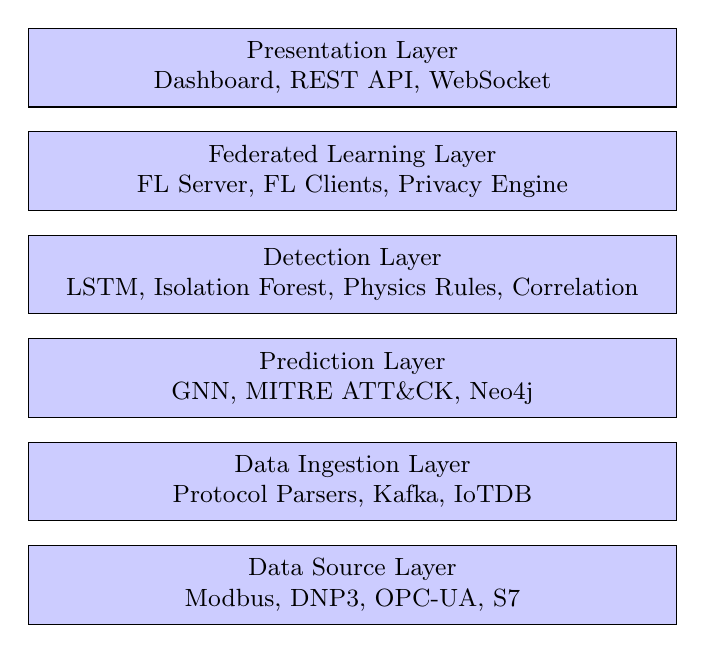
\begin{tikzpicture}[
    node distance=1.5cm,
    layer/.style={rectangle, draw, fill=blue!20, text width=8cm, align=center, minimum height=1cm, font=\small},
    component/.style={rectangle, draw, fill=green!20, text width=3.5cm, align=center, minimum height=0.8cm, font=\scriptsize}
]

\node[layer] (presentation) {Presentation Layer\\Dashboard, REST API, WebSocket};
\node[layer, below=0.3cm of presentation] (fl) {Federated Learning Layer\\FL Server, FL Clients, Privacy Engine};
\node[layer, below=0.3cm of fl] (detection) {Detection Layer\\LSTM, Isolation Forest, Physics Rules, Correlation};
\node[layer, below=0.3cm of detection] (prediction) {Prediction Layer\\GNN, MITRE ATT\&CK, Neo4j};
\node[layer, below=0.3cm of prediction] (ingestion) {Data Ingestion Layer\\Protocol Parsers, Kafka, IoTDB};
\node[layer, below=0.3cm of ingestion] (source) {Data Source Layer\\Modbus, DNP3, OPC-UA, S7};

\end{tikzpicture}
\caption{6-Layer System Architecture}
\end{figure}

\section{Federated Learning Workflow}

\begin{figure}[H]
\centering
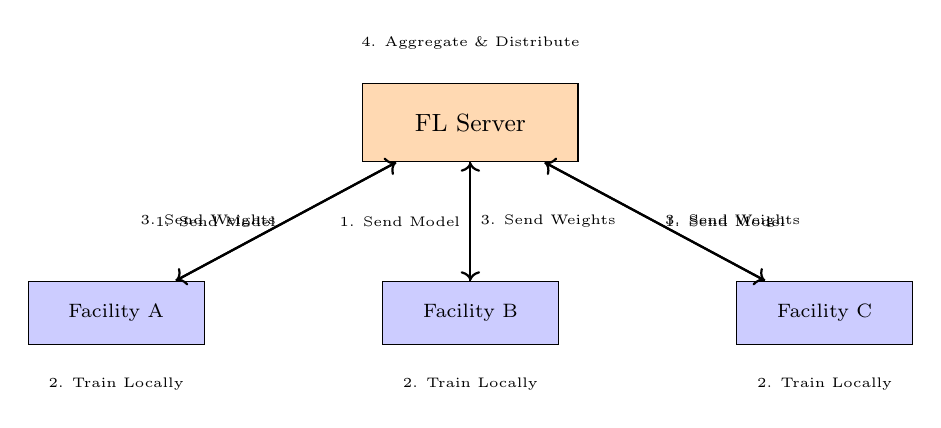
\begin{tikzpicture}[
    node distance=2cm,
    server/.style={rectangle, draw, fill=orange!30, text width=2.5cm, align=center, minimum height=1cm, font=\small},
    client/.style={rectangle, draw, fill=blue!20, text width=2cm, align=center, minimum height=0.8cm, font=\scriptsize},
    arrow/.style={->, thick}
]

\node[server] (server) {FL Server};

\node[client, below left=1.5cm and 2cm of server] (fa) {Facility A};
\node[client, below=1.5cm of server] (fb) {Facility B};
\node[client, below right=1.5cm and 2cm of server] (fc) {Facility C};

\draw[arrow] (server) -- node[left, font=\tiny] {1. Send Model} (fa);
\draw[arrow] (server) -- node[left, font=\tiny] {1. Send Model} (fb);
\draw[arrow] (server) -- node[right, font=\tiny] {1. Send Model} (fc);

\draw[arrow] (fa) -- node[left, font=\tiny] {3. Send Weights} (server);
\draw[arrow] (fb) -- node[right, font=\tiny] {3. Send Weights} (server);
\draw[arrow] (fc) -- node[right, font=\tiny] {3. Send Weights} (server);

\node[below=0.3cm of fa, font=\tiny] {2. Train Locally};
\node[below=0.3cm of fb, font=\tiny] {2. Train Locally};
\node[below=0.3cm of fc, font=\tiny] {2. Train Locally};

\node[above=0.3cm of server, font=\tiny] {4. Aggregate \& Distribute};

\end{tikzpicture}
\caption{Federated Learning Round}
\end{figure}


\section{Performance Metrics}

\begin{table}[H]
\centering
\begin{tabular}{@{}ll@{}}
\toprule
\textbf{Metric} & \textbf{Target Value} \\ \midrule
Detection Latency & $<$30 seconds \\
Detection Accuracy & $>$95\% \\
False Positive Rate & $<$5\% \\
Attack Prediction Accuracy & 67\% \\
Prediction Warning Time & 15-60 minutes \\
Investigation Time Reduction & 80\% \\
MITRE ATT\&CK Coverage & 87\% \\
Threat Propagation Time & 6-24 hours \\
Privacy Guarantee & $\varepsilon=2.0$, $\delta=10^{-5}$ \\
FL Rounds per Day & 4 (every 6 hours) \\
Data Transmitted per Round & $\sim$10 MB \\
Model Accuracy (10 facilities) & 96\% \\
Model Accuracy (50 facilities) & 97\% \\ \bottomrule
\end{tabular}
\caption{Target Performance Metrics}
\end{table}

\section{Competitive Advantages}

\begin{table}[H]
\centering
\small
\begin{tabular}{@{}lll@{}}
\toprule
\textbf{Aspect} & \textbf{Traditional ICS Security} & \textbf{Federated ICS Engine} \\ \midrule
Detection & Signature-based & Multi-source, physics-aware \\
False Positives & 20-30\% & $<$5\% \\
Prediction & None & 67\% accuracy \\
Forensics & Manual (hours) & Automated ($<$30s) \\
Validation & Annual pen tests & Continuous testing \\
Intelligence Sharing & Manual, weeks & Automated, 6-24 hours \\
Privacy & Data exposure & Mathematical guarantees \\
Coverage & Limited & 87\% MITRE ATT\&CK \\ \bottomrule
\end{tabular}
\caption{Competitive Comparison}
\end{table}

\section{Conclusion}

The November 30, 2025 demo must prove the unique value proposition of the Federated ICS Threat Correlation Engine through:

\begin{itemize}[leftmargin=*]
    \item \textbf{Federated Learning:} Collaborative defense across facilities with privacy preservation
    \item \textbf{Multi-Layered Detection:} LSTM, Isolation Forest, and Physics Rules working together
    \item \textbf{Attack Prediction:} Proactive defense using GNN and MITRE ATT\&CK
    \item \textbf{Visual Demonstration:} Real-time dashboard showing all capabilities
    \item \textbf{Privacy Guarantees:} Mathematical proof of data sovereignty
\end{itemize}

\vspace{1cm}

\noindent\textbf{Success Metric:} If federated learning works and demonstrates collaborative defense, the demo succeeds. Everything else enhances but doesn't define success.

\vspace{1cm}

\noindent\rule{\textwidth}{0.4pt}

\noindent\textbf{Document Version:} 1.0 \\
\textbf{Last Updated:} October 14, 2025 \\
\textbf{Status:} Approved for Implementation

\end{document}
